\documentclass[../AnalysisNoteJBuxton.tex]{subfiles}
\begin{document}

\subsection{Results: \texorpdfstring{$\Lambda$K$^{0}_{S}$ and $\Lambda$K$^{\pm}$}{TEXT}}
\label{ResultsLamK}

I first collect all of the summary results, and will show the actual fits to the data in Sections \ref{ResultsLamK_NoRes}, \ref{ResultsLamK_3Res}, and \ref{ResultsLamK_10Res}.  In the first of the summary plots, we show the extracted scattering parameters in the form of a Im[f$_{0}$] vs Re[f$_{0}$] plot, which includes the d$_{0}$ values to the right side.  The next three summary plots show the $\lambda$ vs. Radius parameters.  The first group of plots shows: 1) results without any residual correlations included in the fit (marked as "QM 2017"), 2) results with 10 residual pairs included, and 3) results with 3 residual pairs included.  The second group of plots also includes the case where we fixed the d$_{0}$ parameter to zero.

\begin{figure}[h]
  \centering
  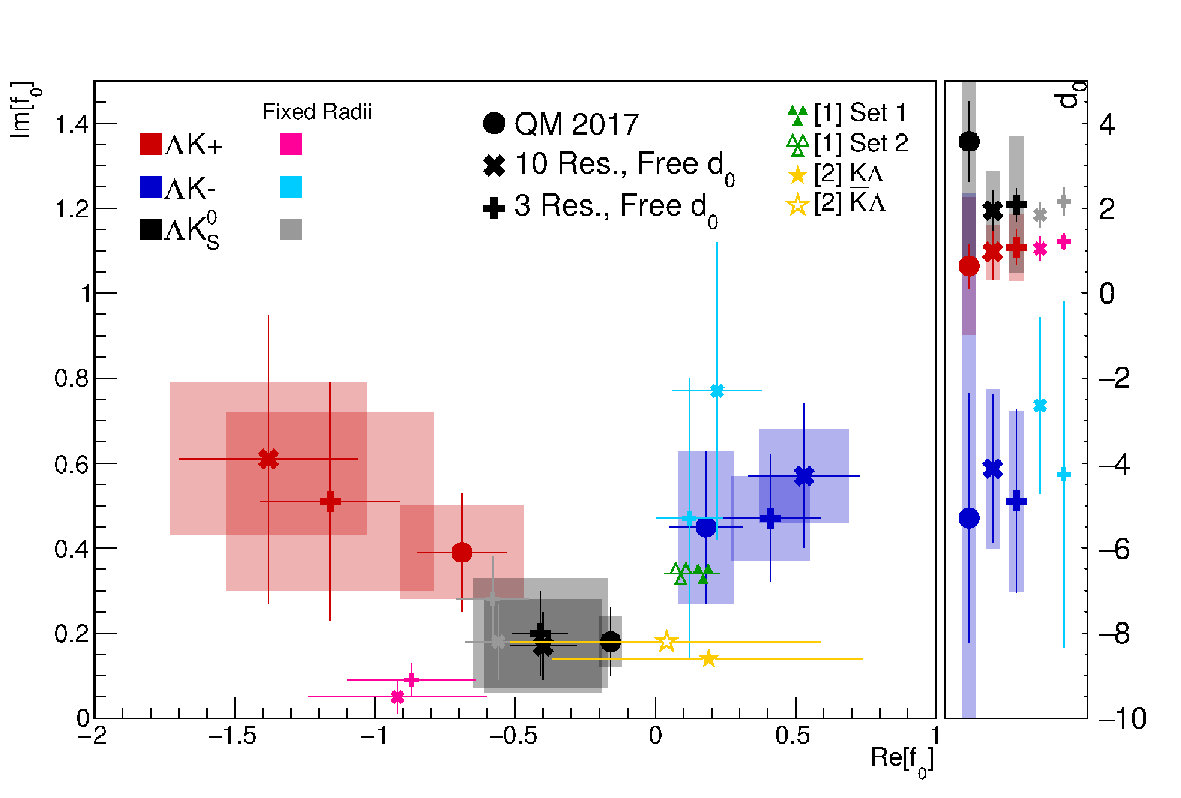
\includegraphics[width=\textwidth]{7_ResultsAndDiscussion/Figures/CompareAllReF0vsImF0AcrossAnalyses_10ResAnd3Res_10and3SeparateOnly_FreeD0Only_wFixedRadiiResults_wScattLenPredictions.pdf}
  \caption[Scattering Parameter Results]{Extracted scattering parameter results, Im[f$_{0}$] vs. Re[f$_{0}$], together with d$_{0}$ to the right, for all of our $\Lambda$K systems.  The plot shows results including no residuals (circles), 10 residual pairs (X), and 3 residual pairs (+).  The lighter color markers (pink, sky blue, gray) show the extracted parameters when we fix the radii to roughly align with the $m_{\mathrm{T}}$-scaling plot, Fig. \ref{fig:mTScalingOfRadii_NoRes}.  The green \cite{Liu:2006xja} and yellow \cite{Mai:2009ce} points show theoretical predictions made using chiral perturbation theory.  Note, $\Lambda$K$^{+}$ on the plot is shorthand for $\Lambda$K$^{+}$ and $\bar{\Lambda}$K$^{-}$, and similar for the others.}
  \label{fig:ImF0vsReF0_FreeD0Only}
\end{figure}


\begin{figure}[h]
  \centering
  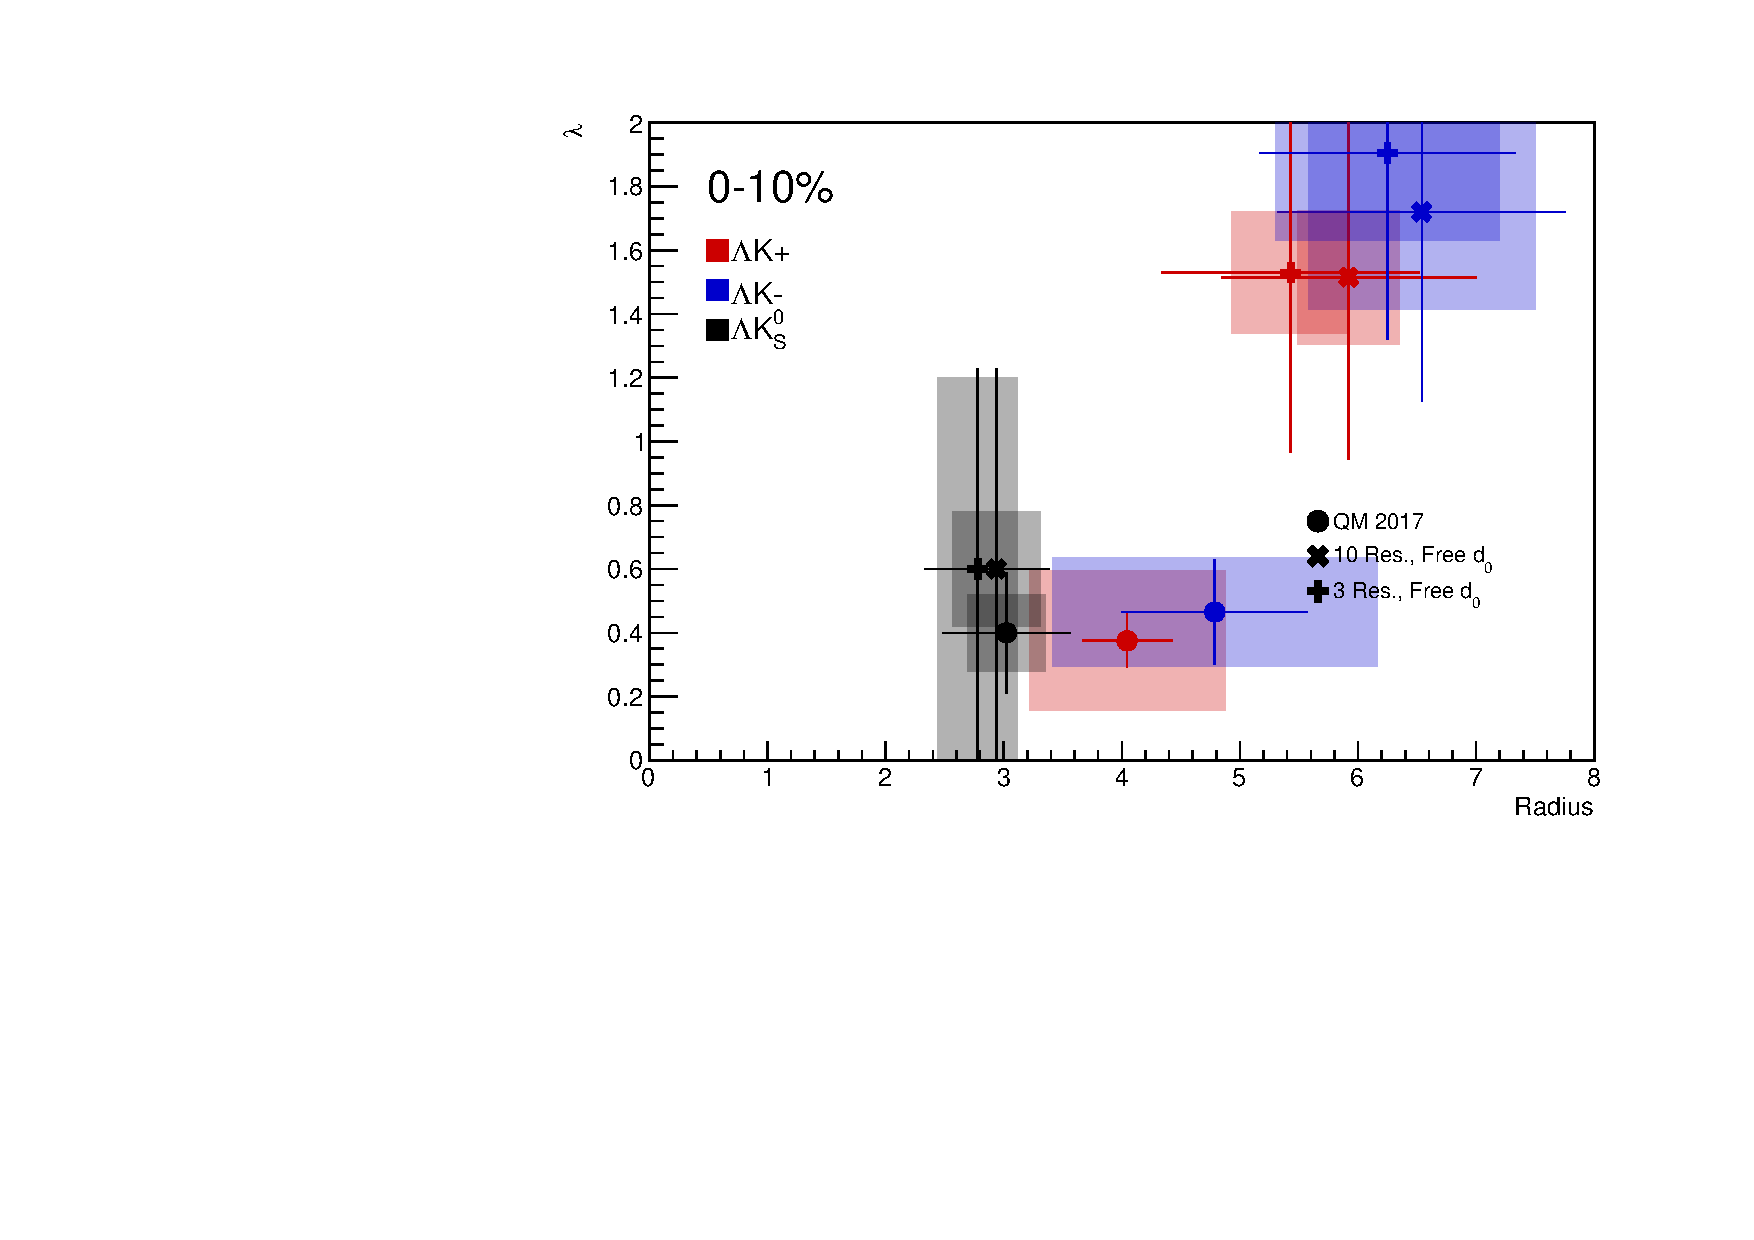
\includegraphics[width=\textwidth]{7_ResultsAndDiscussion/Figures/CompareAllRadiusvsLambdaAcrossAnalyses_0010_10ResAnd3Res_10and3SeparateOnly_FreeD0Only.pdf}
  \caption[$\lambda$ vs. R (0-10\% Centrality)]{Extracted $\lambda$ vs Radius results, for the 0-10\% centrality bin, for all of our $\Lambda$K systems.  The plot shows results including no residuals (circles), 10 residual pairs (X), and 3 residual pairs (+).  Note, $\Lambda$K$^{+}$ on the plot is shorthand for $\Lambda$K$^{+}$ and $\bar{\Lambda}$K$^{-}$, and similar for the others.}
  \label{fig:LambdavsR_0010_FreeD0Only}
\end{figure}

\begin{figure}[h]
  \centering
  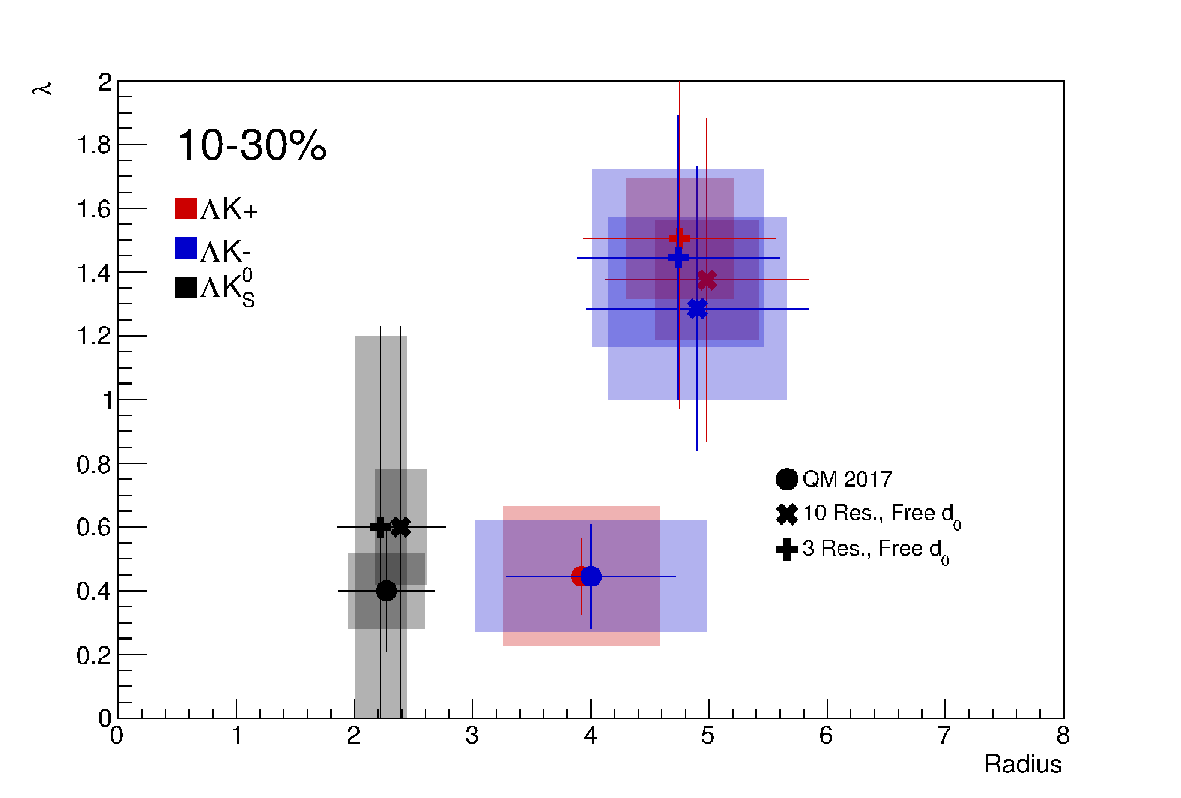
\includegraphics[width=\textwidth]{7_ResultsAndDiscussion/Figures/CompareAllRadiusvsLambdaAcrossAnalyses_1030_10ResAnd3Res_10and3SeparateOnly_FreeD0Only.pdf}
  \caption[$\lambda$ vs. R (10-30\% Centrality)]{Extracted $\lambda$ vs Radius results, for the 10-30\% centrality bin, for all of our $\Lambda$K systems.  The plot shows results including no residuals (circles), 10 residual pairs (X), and 3 residual pairs (+).  Note, $\Lambda$K$^{+}$ on the plot is shorthand for $\Lambda$K$^{+}$ and $\bar{\Lambda}$K$^{-}$, and similar for the others.}
  \label{fig:LambdavsR_1030_FreeD0Only}
\end{figure}

\begin{figure}[h]
  \centering
  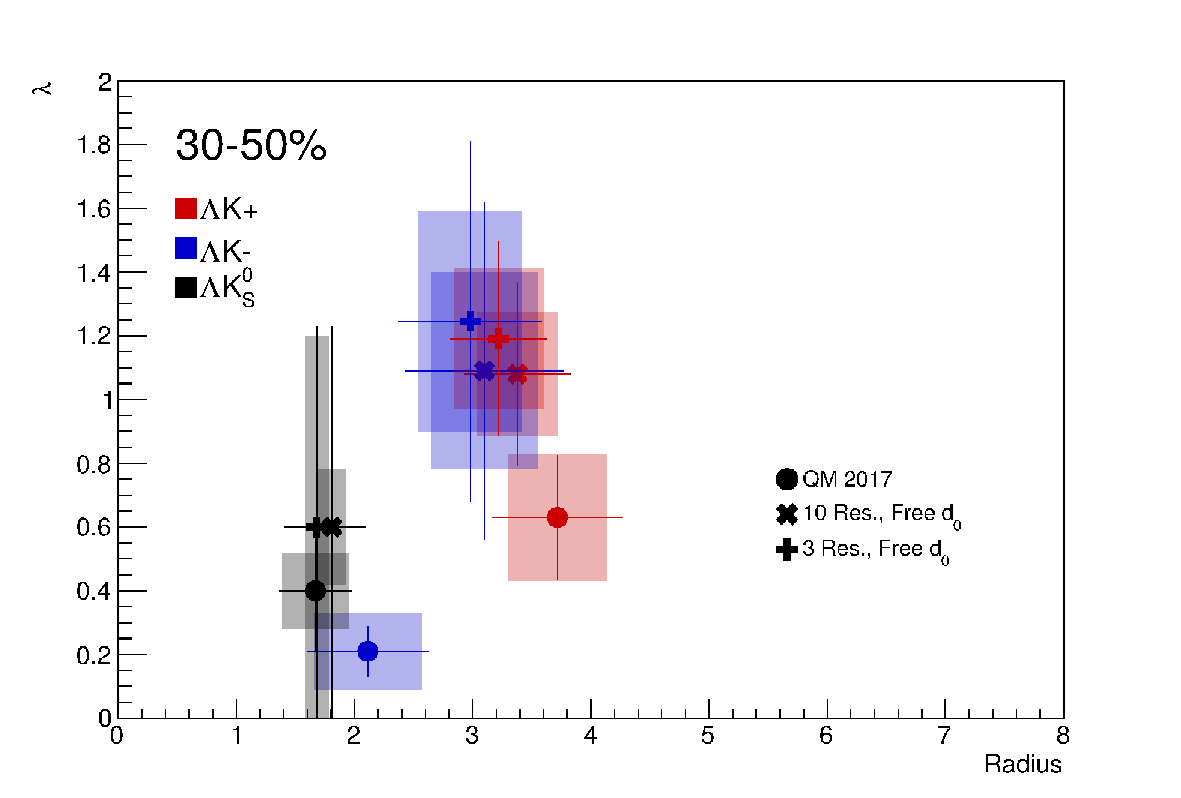
\includegraphics[width=\textwidth]{7_ResultsAndDiscussion/Figures/CompareAllRadiusvsLambdaAcrossAnalyses_3050_10ResAnd3Res_10and3SeparateOnly_FreeD0Only.pdf}
  \caption[$\lambda$ vs. R (30-50\% Centrality)]{Extracted $\lambda$ vs Radius results, for the 30-50\% centrality bin, for all of our $\Lambda$K systems.  The plot shows results including no residuals (circles), 10 residual pairs (X), and 3 residual pairs (+).  Note, $\Lambda$K$^{+}$ on the plot is shorthand for $\Lambda$K$^{+}$ and $\bar{\Lambda}$K$^{-}$, and similar for the others.}
  \label{fig:LambdavsR_3050_FreeD0Only}
\end{figure}










\begin{figure}[h]
  \centering
  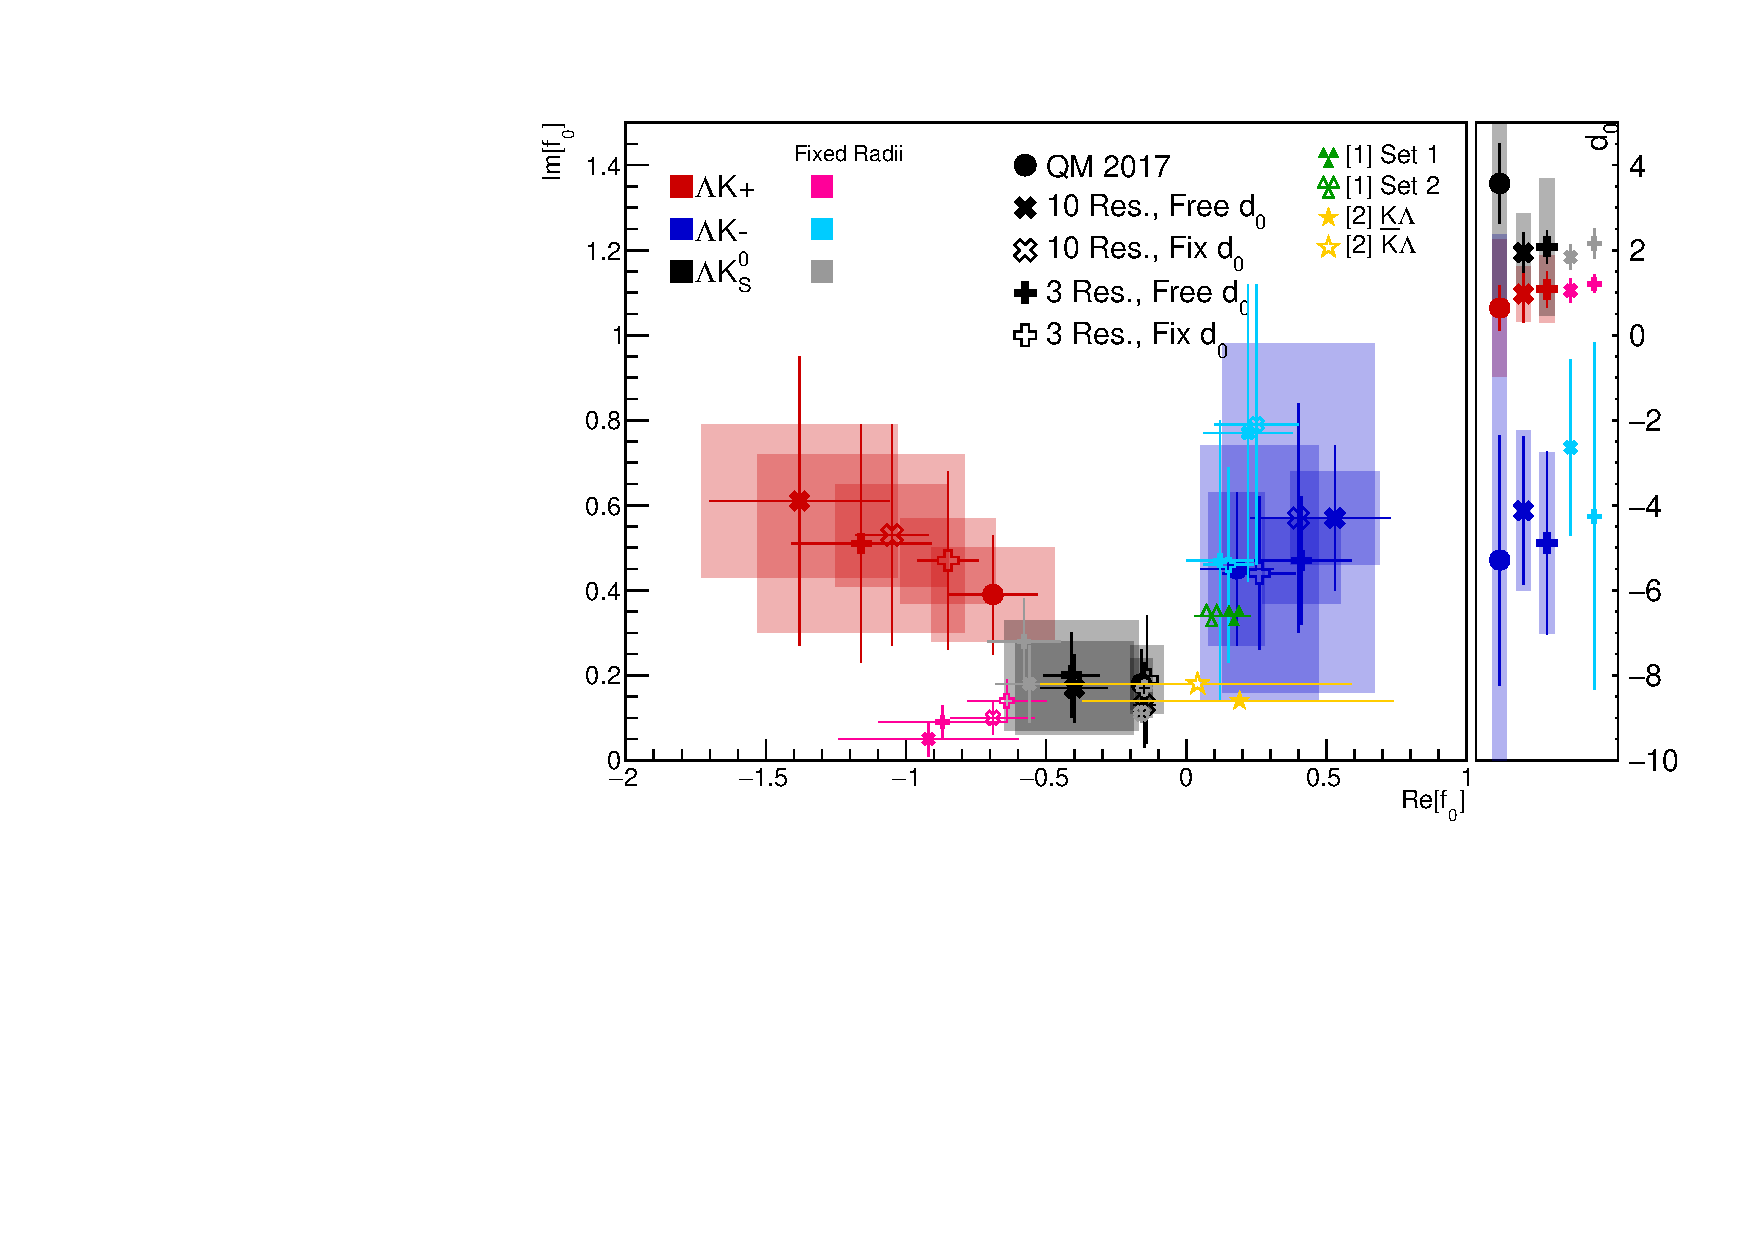
\includegraphics[width=\textwidth]{7_ResultsAndDiscussion/Figures/CompareAllReF0vsImF0AcrossAnalyses_10ResAnd3Res_10and3SeparateOnly_FreeAndFixedD0_wFixedRadiiResults_wScattLenPredictions.pdf}
  \caption[Scattering Parameter Results (free and fixed d$_{0}$)]{Same as Fig. \ref{fig:ImF0vsReF0_FreeD0Only}, but also including the case where d$_{0}$ was fixed to zero in the fit.}
  \label{fig:ImF0vsReF0_FreeAndFixedD0}
\end{figure}

\begin{figure}[h]
  \centering
  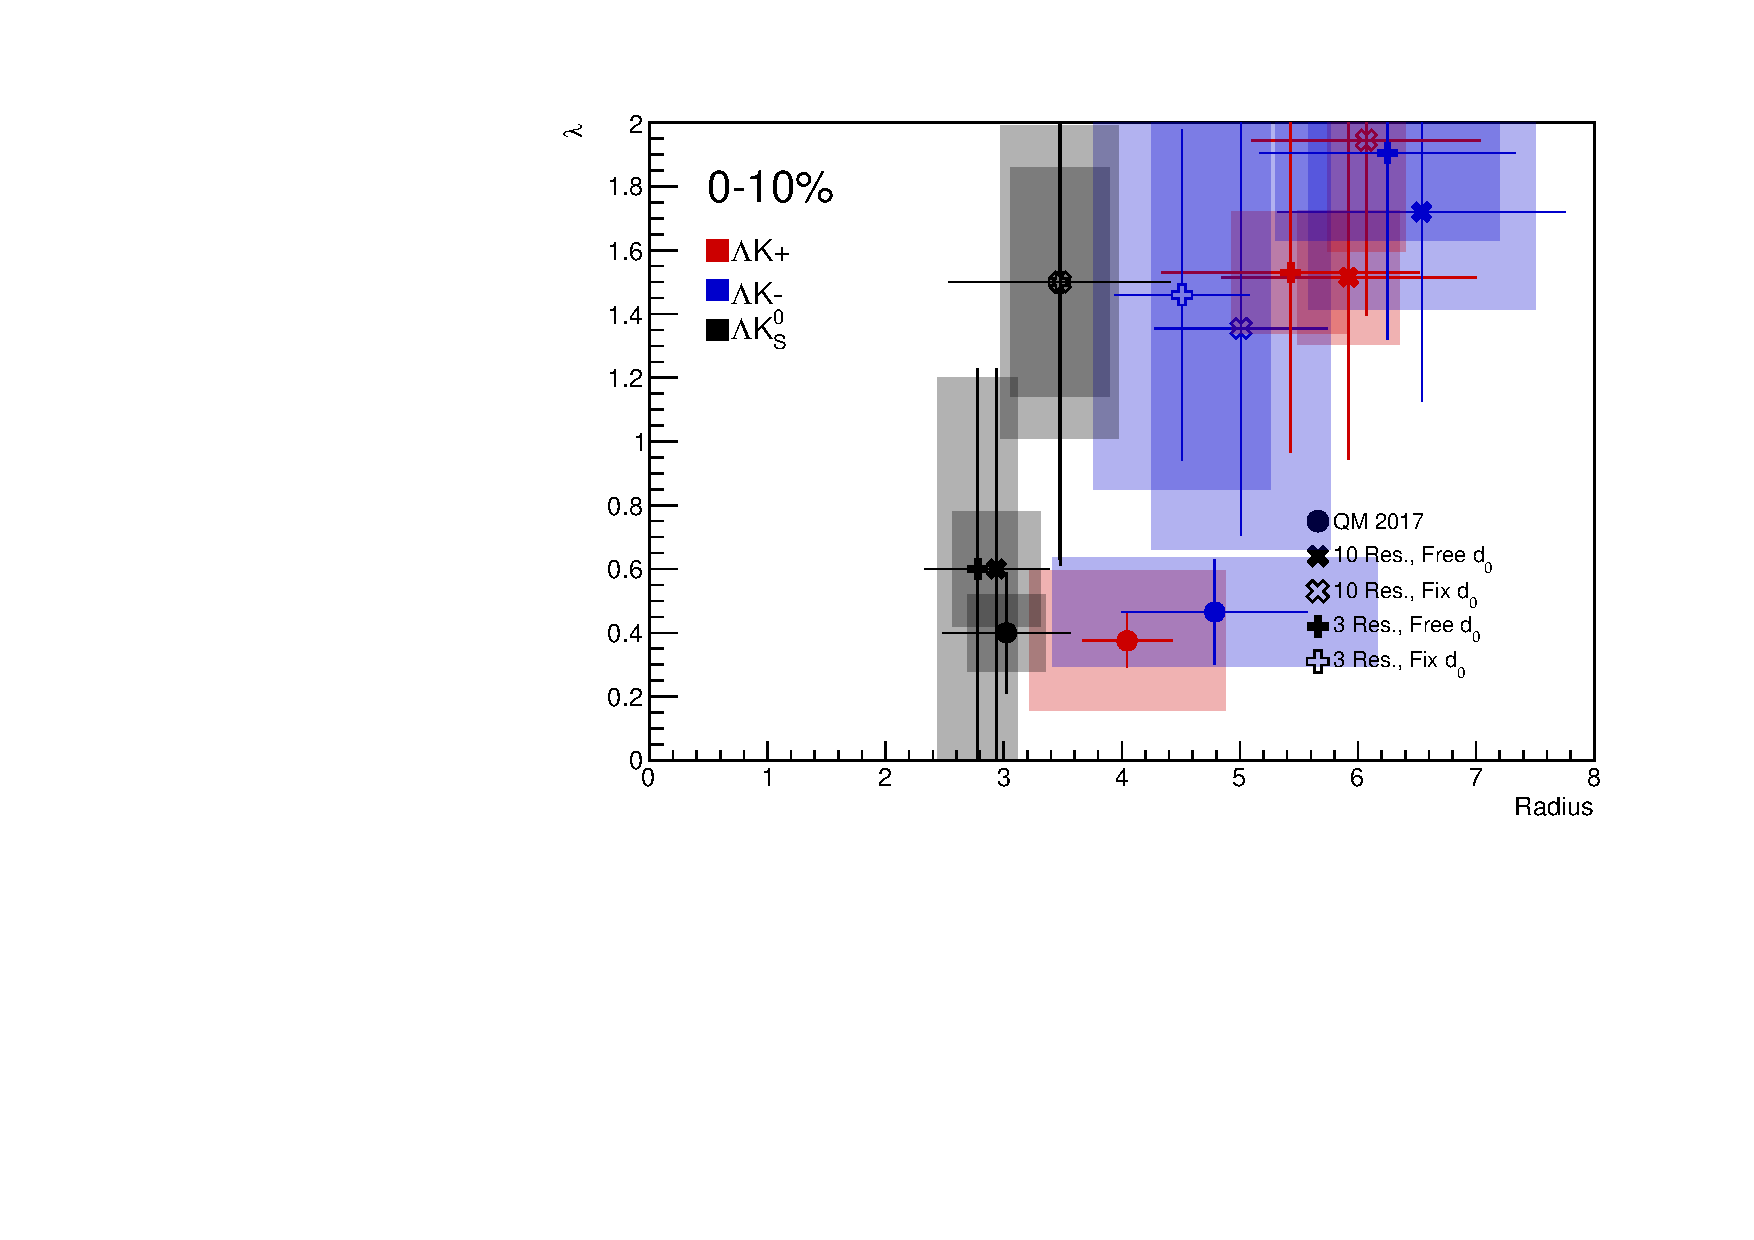
\includegraphics[width=\textwidth]{7_ResultsAndDiscussion/Figures/CompareAllRadiusvsLambdaAcrossAnalyses_0010_10ResAnd3Res_10and3SeparateOnly_FreeAndFixedD0.pdf}
  \caption[$\lambda$ vs. R (0-10\% Centrality) (free and fixed d$_{0}$)]{Same as Fig. \ref{fig:LambdavsR_0010_FreeD0Only}, but also including the case where d$_{0}$ was fixed to zero in the fit.}
  \label{fig:LambdavsR_0010_FreeAndFixedD0}
\end{figure}

\begin{figure}[h]
  \centering
  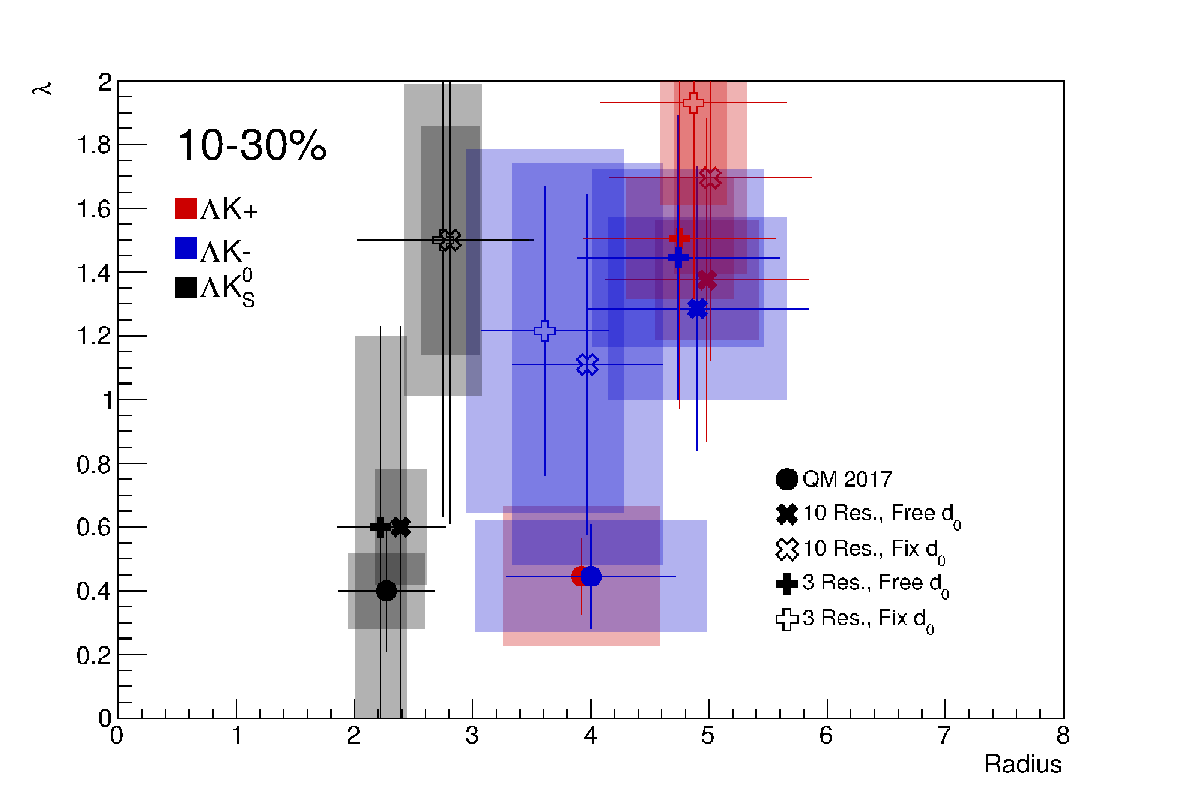
\includegraphics[width=\textwidth]{7_ResultsAndDiscussion/Figures/CompareAllRadiusvsLambdaAcrossAnalyses_1030_10ResAnd3Res_10and3SeparateOnly_FreeAndFixedD0.pdf}
  \caption[$\lambda$ vs. R (10-30\% Centrality) (free and fixed d$_{0}$)]{Same as Fig. \ref{fig:LambdavsR_1030_FreeD0Only}, but also including the case where d$_{0}$ was fixed to zero in the fit.}
  \label{fig:LambdavsR_1030_FreeAndFixedD0}
\end{figure}

\begin{figure}[h]
  \centering
  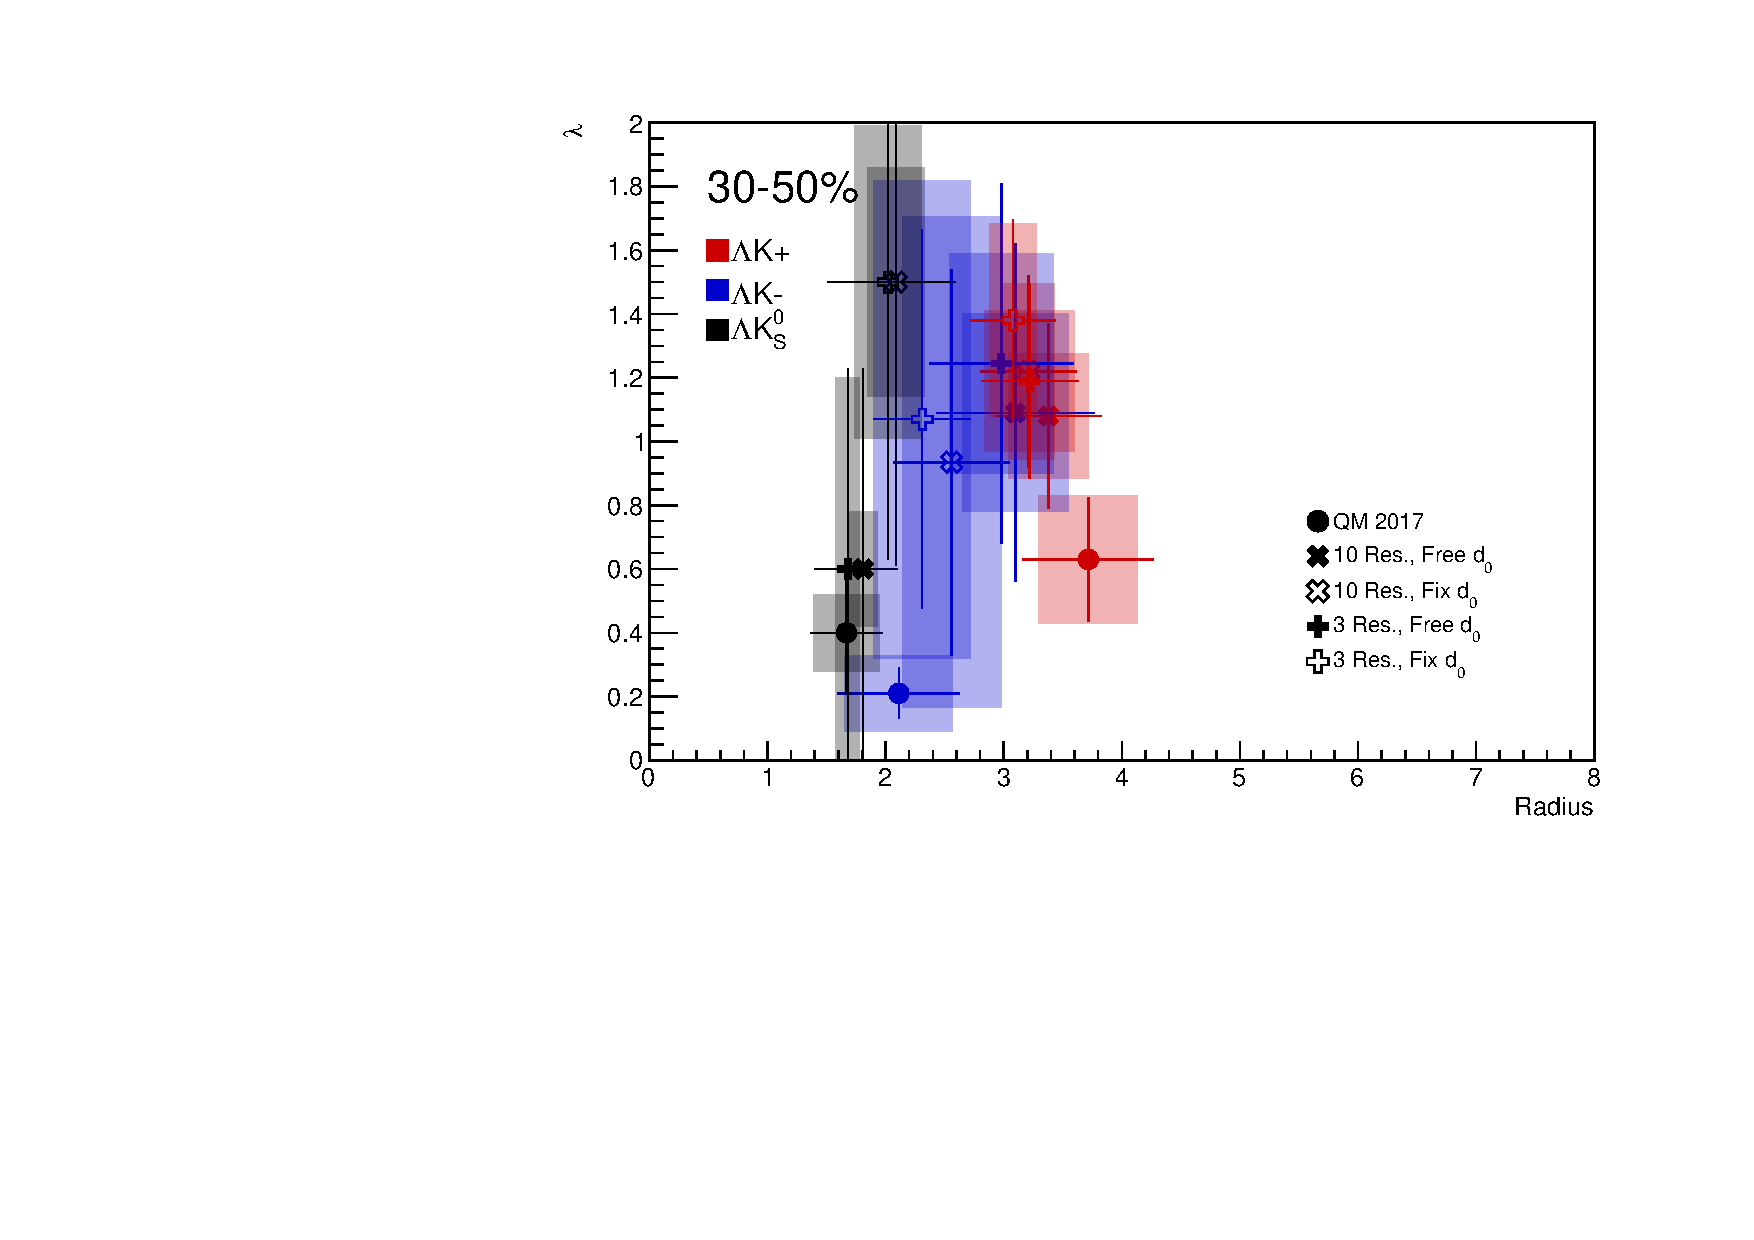
\includegraphics[width=\textwidth]{7_ResultsAndDiscussion/Figures/CompareAllRadiusvsLambdaAcrossAnalyses_3050_10ResAnd3Res_10and3SeparateOnly_FreeAndFixedD0.pdf}
  \caption[$\lambda$ vs. R (30-50\% Centrality) (free and fixed d$_{0}$)]{Same as Fig. \ref{fig:LambdavsR_3050_FreeD0Only}, but also including the case where d$_{0}$ was fixed to zero in the fit.}
  \label{fig:LambdavsR_3050_FreeAndFixedD0}
\end{figure}











\subfile{7_ResultsAndDiscussion/7.1.1_ResultsLamK_NoRes.tex}
\subfile{7_ResultsAndDiscussion/7.1.2_ResultsLamK_3Res.tex}
\subfile{7_ResultsAndDiscussion/7.1.3_ResultsLamK_10Res.tex}

\end{document}